\begin{figure}[!t]
    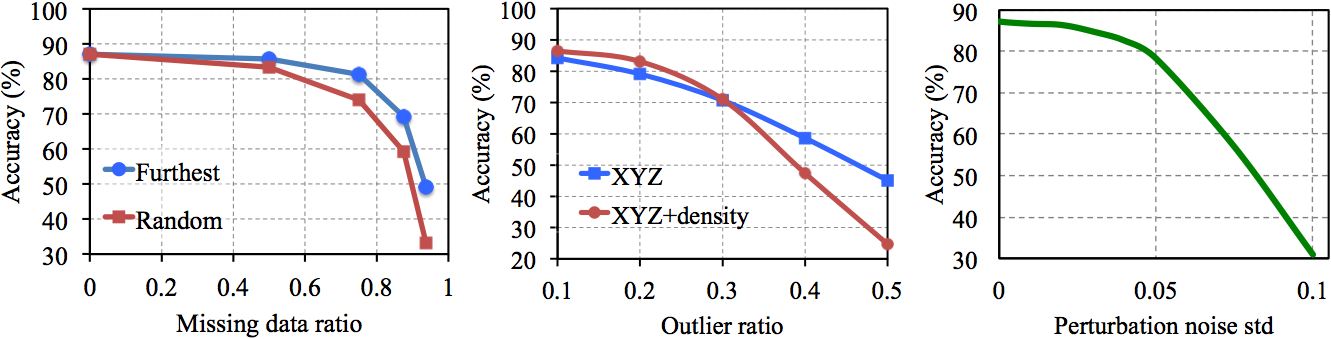
\includegraphics[width=\textwidth]{p51_65}
    \caption{
        \textbf{Robustness tests visualization.}
        Accuracy measured is overall classification accuracy on the ModelNet40
        test set. Left: Point deletion based on different sampling strategies,
        random and furthest sampling, up to the 1024 original points. Middle:
        Insertion of uniformly scattered outliers in the canonicalized unit
        sphere of the original shape. Right: Adding perturbation in the form of
        Gaussian noise with mean 0 to each point in the unit sphere independently.
        Figure from \cite{qi2017pointnet}.
        % The metric is overall classification
        % accuracy on ModelNet40 test set. Left: Delete points. Furthest means
        % the original 1024 points are sampled with furthest sampling. Middle:
        % Insertion. Outliers uniformly scattered in the unit sphere. Right:
        % Perturbation. Add Gaussian noise to each point independently." Figure
        % and caption taken from \cite{qi2017pointnet}. \todo{rewrite in own words}
    } \label{fig:robustness}
\end{figure}


